\documentclass[10pt,twocolumn,twoside]{IEEEtran}

\usepackage{afterpage}
\usepackage{bold-extra}
\usepackage{color}
\usepackage{float}
\usepackage{graphicx}
\usepackage{listings}
\usepackage{subfigure}

%%%%%%%%%%%%%%%
%%% Colours %%%
%%%%%%%%%%%%%%%

\definecolor{darkgreen}{rgb}{0, 0.6, 0}
\definecolor{lightgrey}{gray}{0.9}

%%%%%%%%%%%
% Figures %
%%%%%%%%%%%

% Define shorter ways to include individual images
\newcommand{\stufig}[4]						% images with default placement
{
	\begin{figure}
	\begin{center}
		\includegraphics[#1]{#2}
		\caption{#3}
		\label{#4}
	\end{center}
	\end{figure}
}

\newcommand{\stufigex}[5]					% images with specified placement
{
	\begin{figure}[#5]
	\begin{center}
		\includegraphics[#1]{#2}
		\caption{#3}
		\label{#4}
	\end{center}
	\end{figure}
}

\newcommand{\stufigexx}[5]				% full-width images with specified placement
{
	\begin{figure*}[#5]
	\begin{center}
		\includegraphics[#1]{#2}
		\caption{#3}
		\label{#4}
	\end{center}
	\end{figure*}
}

% Define the stusubfig environment
\newenvironment{stusubfig}[1]
{
	\begin{figure*}[#1]
	\begin{center}
}
{
	\end{center}
	\end{figure*}
}

%%%%%%%%%%%%%%%%%
% Code Listings %
%%%%%%%%%%%%%%%%%

% Create a new type of float (called a stulisting) for listings
\floatstyle{ruled}
\newfloat{stulisting}{thp}{lop}
\floatname{stulisting}{Listing}

% Setup before using the listings package
\renewcommand{\lstlistingname}{\textbf{Listing}}
\def\thelstlisting{\textbf{\arabic{lstlisting}}}

\lstdefinelanguage{Pseudocode}{
morekeywords={and,assert,break,case,continue,default,down,each,else,for,function,if,not,null,or,rangeswitch,ref,return,switch,then,this,throw,to,type,up,var,while},
sensitive=true,
morecomment=[l]{//},
morecomment=[s]{/*}{*/}
}

\lstdefinestyle{Default}{
abovecaptionskip=0.5cm,
basicstyle=\scriptsize\ttfamily,
belowcaptionskip=0.5cm,
belowskip=0.5cm,
columns=fixed,
%commentstyle=\color{darkgreen},
commentstyle=\textit, % changed from the thesis (green text looks unprofessional in a journal paper)
language=Pseudocode,
%numbers=left,
numbers=none, % changed from the thesis (line numbers are less relevant here)
numbersep=5pt,
numberstyle=\tiny,
mathescape=true,
showstringspaces=false,
stepnumber=1,
tabsize=4
}

\lstdefinestyle{Snippet}{
abovecaptionskip=0.5cm,
aboveskip=0.5cm,
basicstyle=\small\ttfamily,
belowcaptionskip=0.5cm,
belowskip=0.5cm,
columns=fixed,
commentstyle=\color{darkgreen},
frame=lines,
keywordstyle=\small\bfseries,
language=Pseudocode,
numbers=none,
mathescape=true,
showstringspaces=false,
stepnumber=1,
tabsize=4
}

% For C++ function prototypes
\lstdefinestyle{Prototype}{
abovecaptionskip=0.5cm,
basicstyle=\small\ttfamily,
belowcaptionskip=0.5cm,
belowskip=0.5cm,
columns=fixed,
commentstyle=\color{darkgreen},
language=C++,
numbers=none,
mathescape=true,
showstringspaces=false,
stepnumber=1,
tabsize=4
}

%%%%%%%%%%%%%%%%%%%%
% Special Commands %
%%%%%%%%%%%%%%%%%%%%

\newcommand{\svlis}{%
\mbox{\scriptsize S\hspace{-0.2mm}\footnotesize V\hspace{-0.2mm}%
\normalsize L\hspace{0.1mm}\footnotesize I\hspace{0.2mm}\scriptsize S\ }}

%%%%%%%%%%%%%%%%%
% Main Document %
%%%%%%%%%%%%%%%%%

\begin{document}

\title{Comparing Partition Forest Segmentations \\ via Slow and Fast Merging}

\author{Stuart~Golodetz, Varduhi~Yeghiazaryan and Irina~Voiculescu%
\thanks{All the authors are with the University of Oxford.}}

\date{\today}

\markboth{IEEE Transactions on Image Processing, Vol.~?, No.~?,~?~2014}%
{Golodetz \MakeLowercase{\textit{et al.}}: Comparing Partition Forest Segmentations via Slow and Fast Merging}

\IEEEpubid{0000--0000/00\$00.00~\copyright~2014 IEEE}

\maketitle

\begin{abstract}
\noindent TODO
\end{abstract}

\begin{IEEEkeywords}
abdominal CT scans, image partition forests, multi-rate merging, segmentation comparison
\end{IEEEkeywords}

\IEEEpeerreviewmaketitle

%#####################
\section{Introduction}
%#####################

TODO: \cite{golodetz11}

\textbf{In this paper, we present the slow and fast forest merging methods for a pair of partition forests over the same base image. We further show how the resulting merged forests can be compared straightforwardly to characterise the similarity between the original forests.}

The organisation of this paper is as follows: in \S\ref{sec:ipfs}, we briefly revisit the concept of an image partition forest; in \S\ref{sec:merging}, we present our merging methods; in \S\ref{sec:comparisons}, we present various ways in which the merged forests can be compared; in \S\ref{sec:experiments}, we evaluate the effectiveness of our comparison approaches on some popular test images from the literature; and in \S\ref{sec:discussion}, we analyse the results of our experiments.

%################################
\section{Image Partition Forests}
\label{sec:ipfs}
%################################

TODO

\stufigex{width=.75\linewidth}{ipfs-concept.png}{The concept of a partition forest (see \S\ref{sec:ipfs} for discussion)}{fig:ipfs-concept}{!t}

%#######################
\section{Forest Merging}
\label{sec:merging}
%#######################

Merging two partition forests together conceptually entails merging the corresponding layers in the two forests together and connecting the results. Since each partition forest layer is a mosaic image, merging two such layers together involves combining mosaics (see Figure~\ref{?}). This can be done in one of two ways, giving differing results: one way is to add an edge to the output image iff either input image contains the edge (see Figure~\ref{?}); the other is to add an edge to the output image only iff both input images contain the edge (see Figure~\ref{?}). Note that the first way results in an output image that allows us to express every region in either input image as a union of regions in the output. For the rest of this paper, we will call the first way \emph{slow merging} and the second way \emph{fast merging} (expressing a reluctance to merge regions in the former case and an eagerness to do so in the latter). We call the partition forest resulting from combining the corresponding layers of the input forests using slow (respectively fast) merging the \emph{slow (respectively fast) merged forest}.

TODO

\subsection{Building Common Ancestor Tables (CATs)}

TODO

%---
\begin{stulisting}[t]
\caption{Building a Common Ancestor Table}
\label{code:build-cat}
\lstinputlisting[style=Default]{build-cat.lst}
\end{stulisting}
%---

\subsection{Slow and Fast Merging}

TODO

%---
\begin{stulisting}[t]
\caption{Building a Slow CAT}
\label{code:build-slow-cat}
\lstinputlisting[style=Default]{build-slow-cat.lst}
\end{stulisting}
%---

\subsection{Building Merge Tables}

TODO

%---
\begin{stulisting}[t]
\caption{Building a Merge Table}
\label{code:build-merge-table}
\lstinputlisting[style=Default]{build-merge-table.lst}
\end{stulisting}
%---

\IEEEpubidadjcol

\subsection{Building the Merged Forests}

TODO

%---
\begin{stulisting}[t]
\caption{Building the Merged Forests}
\label{code:build-merged-forest}
\lstinputlisting[style=Default]{build-merged-forest.lst}
\end{stulisting}
%---

%---
\begin{stusubfig}{!t}
	\subfigure[Forest X]{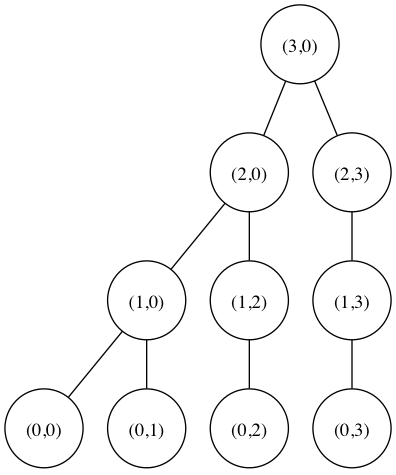
\includegraphics[width=.22\linewidth]{merging-example-a.png}}%
	\hspace{4mm}%
	\subfigure[Forest Y]{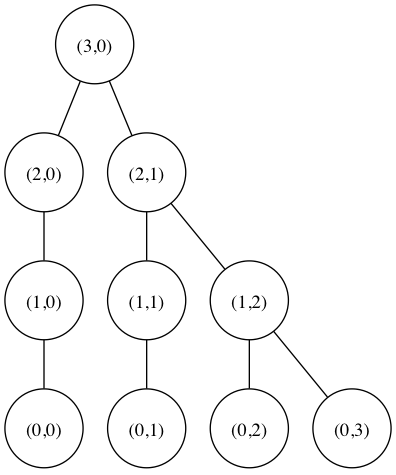
\includegraphics[width=.22\linewidth]{merging-example-b.png}}%
	\hspace{4mm}%
	\subfigure[SlowMerge(X,Y)]{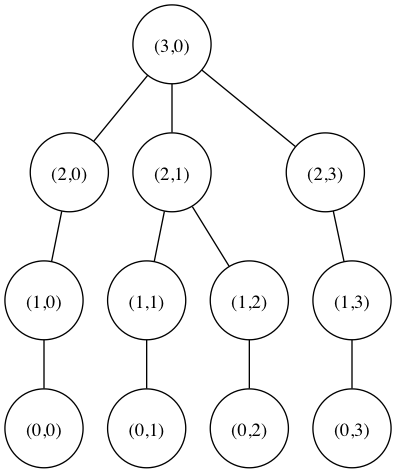
\includegraphics[width=.22\linewidth]{merging-example-c.png}}%
	\hspace{4mm}%
	\subfigure[FastMerge(X,Y)]{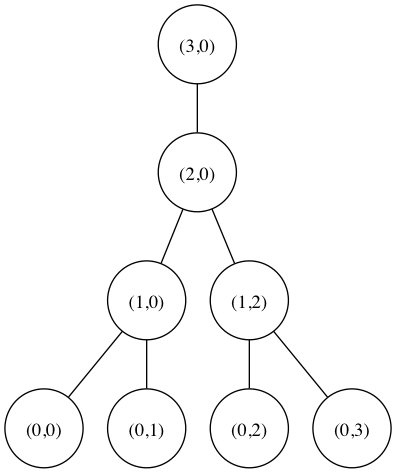
\includegraphics[width=.22\linewidth]{merging-example-d.png}}%
\caption{TODO}
\label{fig:merging-example}
\end{stusubfig}
%---

%################################
\section{Comparing Segmentations}
\label{sec:comparisons}
%################################

TODO

%######################
\section{Experiments}
\label{sec:experiments}
%######################

TODO

%#####################
\section{Discussion}
\label{sec:discussion}
%#####################

TODO

%######################
\section{Conclusions}
\label{sec:conclusions}
%######################

TODO

%#########################
\section{Acknowledgements}
%#########################

We remain profoundly grateful to Dr.\ Zoe Traill of the Churchill Hospital, Oxford, both for providing us with abdominal CT scans and for giving up her time to help us interpret them. We also gratefully acknowledge the past support of the UK Engineering and Physical Sciences Research Council (EPSRC) in funding Stuart Golodetz's doctoral work via a Doctoral Training Account (DTA).

\clearpage

\bibliographystyle{alpha}
\bibliography{existingwork,mypapers}

\vspace{3cm}

\begin{IEEEbiography}[{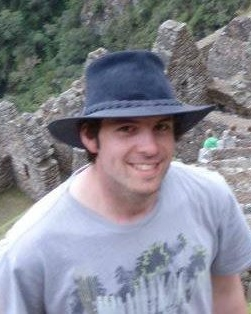
\includegraphics[width=1in,height=1.25in,clip,keepaspectratio]{pic_stuart.jpg}}]{Stuart Golodetz}
obtained his DPhil in Computer Science at the University of Oxford, working on 3D image segmentation and feature identification. After spending two interesting years in industry, working in the areas of credit risk management, logic programming and software analytics, he is now working as a Research Associate at the University of Oxford. His areas of interest include medical image analysis, computer games development and the intricacies of different programming languages, especially C++. He was a session chair for the 6th International Symposium on Image and Signal Processing and Analysis, ISPA 2009. He is a member of the Association of C and C++ Users (ACCU) and has written a number of articles for their magazines.
\end{IEEEbiography}

\begin{IEEEbiography}[]{Varduhi Yeghiazaryan}
TODO
\end{IEEEbiography}

\begin{IEEEbiography}[{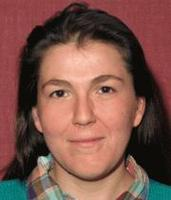
\includegraphics[width=1in,height=1.25in,clip,keepaspectratio]{pic_irina.jpg}}]{Irina Voiculescu}
is a Lecturer in Computer Science at the University of Oxford. She obtained a PhD at the University of Bath, for research in Constructive Solid Geometry. She contributed to the development of the geometric modelling software \svlis through the application of polynomial root finding methods. She works in the general area of geometric modelling, specifically focusing on the mathematics of curves and surfaces, interval arithmetic, molecular modelling and medical image analysis. She is a Fellow of the UK Geometric Modelling Society.
\end{IEEEbiography}

\end{document}
